%%==================================================
%% chapter01.tex for BIT Master Thesis
%% modified by yang yating
%% version: 0.1
%% last update: Dec 25th, 2016
%%==================================================
\chapter{绪论}
\label{chap:intro}
\section{研究背景与意义}
代码克隆,也叫代码复用,是指在软件系统中存在两个或两个以上的相似代码片段\cite{乐乔艺2021代码克隆检测研究进展综述},是软件开发中的常见现象。随着互联网时代的发展,网络上各种开源项目越来越多样化,获取也更加便利。许多企业通过软件资源库、外部开源软件、软件产品线及开发框架等多种方式建立了多种多样的软件复用开发方法,同时开发人员自身也会通过多种方式大量复用已有的软件资源。在这些软件复用方法和资源的支持下,软件系统和软件产品大量引入了开源软件、网络资源、商业软件等第三方代码成分。这些第三方代码在多个软件系统中复制、传播和演化,给软件系统带来了软件质量的不确定性和风险,甚至导致漏洞的传播。

近年来第三方代码中包含的漏洞数量呈现出快速增长的趋势。根据美国新思科技公司(Synopsys, Inc.)发布的《2023年开源安全和风险分析报告》\cite{Synopsys_2023}显示,在2022年审计的1703个代码库中,98\%的项目都包含开源代码,84\%的代码库包含至少一个已知开源漏洞,比2022年版的报告中增加了近4\%,有48\%代码库中包含高风险漏洞。
图\ref{fig:Proportion}统计了2018年至2022年Synopsys审计代码库中开源代码及漏洞占比,从图中可以看出开源代码及漏洞数量整体呈上升趋势。
\begin{figure}
 \centering
 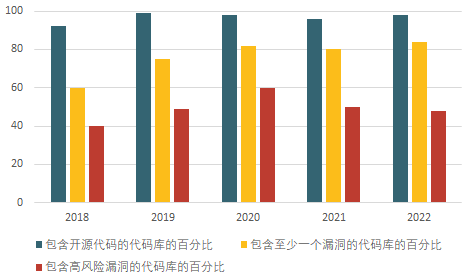
\includegraphics[width=0.75\textwidth]{figures/Proportion}
 \caption{2018-2022年Synopsys审计代码库中的开源代码及漏洞占比示意图}
 \label{fig:Proportion}
\end{figure}
同时,Synopsys统计了包含易受攻击组件的代码库占比,其中使用JQuery 和 Lodash 两个最流行的开源组件的代码库占比达到了47\%和 31\%,其余组件占比如图\ref{fig:assembly}所示。
\begin{figure}
    \centering
    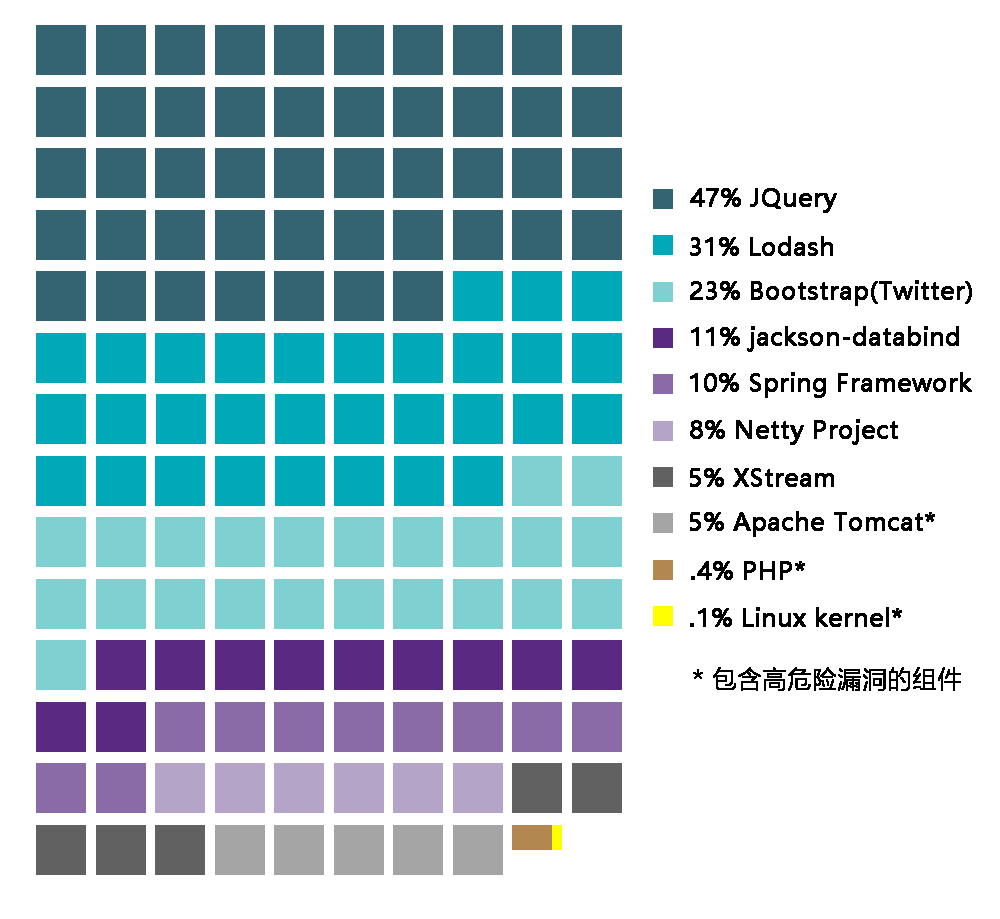
\includegraphics[width=0.75\textwidth]{figures/assembly}
    \caption{2022年Synopsys审计代码库中包含易受攻击组件的百分比示意图}\label{fig:assembly}
\end{figure}
据Gartner\cite{Gartner_2022}预测,到2025年,全球45\%的组织将遭受软件供应链攻击,比2021年增加三倍。因此,准确地检测代码克隆对于软件开发和维护是至关重要的。

早期代码克隆检测技术通常将代码视为自然语言文本进行处理,通过文本相似性判断代码相似程度;随着编译技术的发展,研究者们将编译原理中的词法分析技术运用到代码克隆检测领域;近年来,基于多维源代码表征学习的代码克隆检测技术已经引起了学者们广泛的兴趣,有研究人员从代码克隆检测与代码表征学习技术相结合这一方面进行了探索,试图从关键技术点入手,找到合适的结合点,以提高定代码克隆检测技术的效率和智能化程度。


\section{研究现状与趋势}

\subsection{代码克隆检测技术概述}
%\label{sec:features}
代码克隆检测技术,旨在自动化定位软件系统中的代码克隆,节省成本,减少出错风险,有助于更好地保证软件质量。目前已有的代码克隆方法大多需要对代码片段进行信息抽取,转换为中间表征,然后根据表征方式的不同计算不同代码片段之间的相似度,完成克隆检测任务。其具体流程如图\ref{fig:figure1}所示。
\begin{figure}
    \centering
    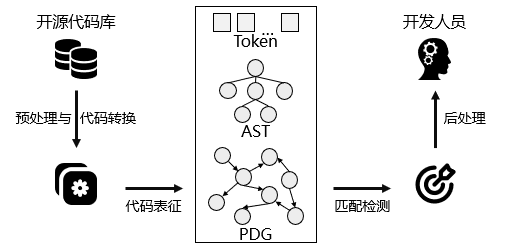
\includegraphics[width=0.95\textwidth]{figures/figure1}
    \caption{代码克隆检测流程}\label{fig:figure1}
\end{figure}

从图\ref{fig:figure1}可以看出一个完整的代码克隆检测过程通常包括预处理、代码转换、表征学习、匹配检测、后处理几个阶段。具体而言,一般的代码克隆检测从代码预处理开始,首先删除与检测无关的空白行、注释、缩进等元素,并根据检测粒度将源代码划分为单独的片段,比如类、函数等;然后将比较单元转化为相应的中间表示,常见的中间表示有:词法单元(Token)、抽象语法树(abstract syntax tree,AST)、程序依赖图(Program dependency graph,PDG)等;在表征学习阶段,将根据上一阶段得到的中间表示采用相应的匹配算法进行相似度计算,例如抽象语法树的比较通常采用子树匹配算法,程序依赖图的比较则采用子图同构算法。此阶段将代码片段两两对比,以查找相似代码源片段,得到代码克隆对。

在这些步骤中,源代码表征方式决定了检测方法的预处理方式、模型设计、部署方式、运行效率,并影响最终结果[2]。

代码克隆检测和代码表征学习之间存在密切的关系。代码表征学习是指利用机器学习或深度学习技术从源代码中学习有效的表示,以便于后续的软件工程任务,如代码克隆检测、代码推荐、缺陷预测等。

在代码克隆检测中,代码表征学习可以用来提取代码片段的特征表示,这些特征表示能够捕捉代码的语法、语义以及结构信息。通过学习到的代码表征,我们可以更准确地比较和识别不同代码片段之间的相似性,从而实现克隆代码的检测和管理。

常见的代码表征学习方法包括基于深度学习的方法,如卷积神经网络(CNN)、循环神经网络(RNN)、注意力机制等。这些方法可以从源代码中学习到高层次的抽象特征表示,使得克隆代码检测可以在更抽象的层次上进行,从而提高检测的准确性和鲁棒性。

因此,代码表征学习为代码克隆检测提供了重要的技术支持,它使得我们能够更有效地利用机器学习和深度学习技术来处理大规模的代码库,并提高代码克隆检测的性能和效率。

因此源代码表征学习是代码克隆检测的关键步骤。

\subsection{代码表征学习}



\section{研究内容}

代码克隆检测是软件工程领域一项重要任务,如何对代码进行合适的表征是代码克隆检测的关键问题。代码表征学习决定了对源代码信息抽取程度的上限,决定了检测技术的预处理方法、模型设计、部署方式、运行效率,并会影响最终结果。面向代码克隆检测这一下游任务,代码表征学习研究存在以下不足:对代码结构信息语义信息利用不充分,特征表达不够完善;表征模型对数据集、模型结构和优化算法等多方面因素的要求高等问题,这些不足严重制约着代码克隆检测技术的发展。因此,研究人员一方面通过对源代码进行充分利用,提出多维源代码表征方法,从而提高代码克隆检测能力;另一方面,通过研究更先进的算法来提高表征模型的自动化和智能化程度,也是目前重要的发展趋势。

本文的主要工作包括:

(1)提出面向代码克隆检测的多维源代码表征学习方法 

针对现有代码表征学习方法存在的对代码结构信息和语义信息利用不充分、表征模型对数据集依赖过高等问题,本文提出面向代码克隆检测的多维源代码表征学习方法,旨在通过构建三个不同维度的代码表征模型,将源代码的语义信息表示为稠密低维实值向量,以在低维空间中高效计算实体和关系的语义联系,并通过特征融合得到多维特征,实现对代码信息的充分利用,以更加全面准确与智能化的方式提高代码克隆测试效率。

(2)面向集外词问题的Token表征学习

具体的,针对Token序列特征挖掘,提出预训练增强辅助模型提取属性特征,从而解决传统基于Token序列的方法存在的集外词问题;
针对抽象语法树AST特征挖掘,提出子树划分的改进方法提取结构特征,从而解决传统基于抽象语法树的方法存在的梯度消失问题;
针对程序依赖图PDG特征挖掘,提出过滤机制提取语义特征,通过收集PDG的简单特征来过滤掉明显不可能为克隆的PDG对,从而解决传统基于程序依赖图的方法存在的计算开销大问题。
针对不同的特征采用不同的代码表征模型对代码片段进行多维源代码特征学习,从而提高对源代码特征提取的程度,并通过特征融合得到一个更能代表代码信息的多维特征,该多维特征能够在低维空间中高效计算实体和关系的语义联系,提高后续代码克隆检测任务的准确率。

(3)实验评估

如图\ref{fig:diagram}所示

\begin{figure}
 \centering
 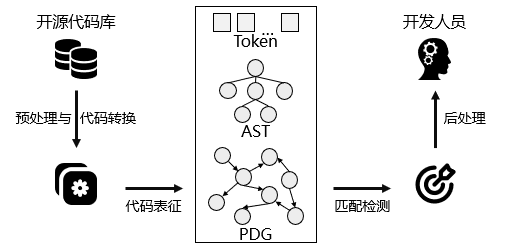
\includegraphics[width=0.75\textwidth]{figures/figure1}
 \caption{热塑性形状记忆聚氨酯的形状记忆机理示意图}\label{fig:diagram}
\end{figure}


\section{论文结构}
%\label{sec:requirements}
本文围绕三个关键技术点展开研究,论文后续各章节具体内容如下:
第1章 绪论 该部分对本文的研究背景与意义进行了阐述 
第2章 从
第3章 介绍基于预训练辅助模型的Token表征学习方法的设计与实现。
第4章 介绍基于子树划分的抽象语法树表征学习方法设计与实现。
第5章 介绍基于图过滤的程序依赖图表征学习方法设计与实现。
第6章 本文研究框架RLCCD的实验验证。
结论 对全文的研究进行了总结,并提出对未来工作的展望。

\cite{Jiang2005Size} ,如表 \ref{tab:category}所示。
